\documentclass[10pt,a4paper,onecolumn]{article}
\usepackage[usenames,dvipsnames]{color}
\usepackage[colorlinks,citecolor=blue]{hyperref}
\usepackage{appendix}
% we need umlauts in the refs
\usepackage[english]{babel}
\usepackage[utf8]{inputenc}
\usepackage[T1]{fontenc}

%\usepackage[natbib=true,style=authoryear,backend=biber]{biblatex}
\usepackage{authblk}
\renewcommand\Affilfont{\itshape\small}
\usepackage{graphicx}
\usepackage[authoryear]{natbib}
\usepackage{url}
\usepackage{todonotes}
%\usepackage{endfloat}
% nicer units
\usepackage{units}
% better tables
\usepackage{booktabs}
% Some colorings for the tables
%\usepackage[table]{xcolor}

%\usepackage{multirow}

% switch for final stage
%\graphicspath{{pics/}}
\graphicspath{{pics/}
              {pics/generated/}}

%\usepackage{lineno}
%\usepackage[leftbars]{changebar}
%\setlength\changebarsep{0.5em}
%\usepackage{comment}

%\usepackage[space]{grffile}
%\usepackage{latexsym}
%\usepackage{amssymb}
%\usepackage{fancyref}
\usepackage{textcomp}

\usepackage{marvosym}
\usepackage{listings}

\lstset{prebreak=\Righttorque}
\lstset{postbreak=\Lefttorque}
\lstset{breakindent=0pt}
\lstset{frame=lines}
\lstset{aboveskip=4mm}
\lstset{breaklines=true, breakatwhitespace=false}
\urlstyle{same}
% howto cite projects
\newcommand{\purl}[2]{#1\footnote{\url{#2}}}

\newcommand{\sevenT}{\unit[7]{Tesla}}
\newcommand{\threeT}{\unit[3]{Tesla}}
\newcommand{\mm}[1]{\unit[#1]{mm}}
\newcommand{\seconds}[1]{\unit[#1]{s}}

\newcommand{\ie}[0]{\emph{i.e.},\ }
\newcommand{\eg}[0]{\emph{e.g.},\ }
\newcommand{\etc}[0]{\emph{etc.}}

\begin{document}
\bibliographystyle{unsrt}

\title{The encoding encyclopedia}


\author[1]{Moritz~Boos}
\author[2]{J.~Swaroop~Guntupalli}
\author[3,4]{Michael~Hanke}

\affil[1]{Oldenburg, Germany}
\affil[2]{Department of Psychological and Brain Sciences,
  Dartmouth College, Hanover, New Hampshire, USA}
\affil[3]{Psychoinformatics lab, Department of Psychology II, University of
Magdeburg, Magdeburg, Germany}
\affil[4]{Center for Behavioral Brain Sciences, Magdeburg, Germany}
\maketitle
\thispagestyle{fancy}

\listoftodos

\begin{abstract}
% Abstracts should be up to 300 words and provide a succinct summary of the
% article. Although the abstract should explain why the article might be
% interesting, care should be taken not to inappropriately over-emphasise the
% importance of the work described in the article. Citations should not be used
% in the abstract, and the use of abbreviations should be minimized.

\todo[inline]{find title}
\todo[inline]{write abstract}
\end{abstract}

\clearpage


\section*{Introduction}

\cite{CTK+2012}

\todo[inline]{any fieldstrength differences, i.e. higher resolution gives better model?}
\todo[inline]{formisano says 7T better, but more stimuli and more data with a different model are confounds}
\todo[inline]{unclear which quality metric is most appropriate due to lack of literature}
\todo[inline]{maybe add other feature sets and check metrics across all of them}

% summary: first comparative study

\todo[inline]{is this the first decode(encode(fmri)) study?}

\section*{Methods}

\cite{HBI+14,HDH+2015}

\subsection*{fMRI data}

\paragraph{\unit[3]{Tesla}}
\paragraph{\unit[7]{Tesla}}

\subsection*{Encoding model}

\todo[inline]{reference feature set description and describe encoding algorithm}

\missingfigure{encoding scheme}

%each voxel separately, ridge, generalized cross-validation -- look up possible citations

For each f{MRI} sample $y_{vt}$ (where $t=1,2,..,T$ denotes the time-points and $v=1,2,..,V$ denotes the voxels) the LQ-MFS features $x_{t}$ $[1x\widetilde{M}]$ (where $\widetilde{M}$ is the number of LQ-MFS coefficients) of the corresponding two second part of the stimulus were computed. In case there was no stimulus presented at time-point $t$, it was associated with a $[1x\widetilde{M}]$ zero-vector. 

%make more clear that notation is overloaded
Since the BOLD response is delayed, for each f{MRI} sample, the most recent feature was vector removed (since it could not yet have influenced the f{MRI} activity), and the new feature vector at time-point $t$ was created by concatenating the prior feature vectors $x_{t-1}$,$x_{t-2}$ and $x_{t-3}$, further denoted as $x_{t}$. Time-points were removed from the analysis, if two-thirds or more of the concatenated feature vectors were zero-vectors.

The f{MRI} activity time-series, as well as the feature time-series, were then vertically stacked, resulting in a matrix of features $X$ $[NxM]$ (where $N$ is the number of f{MRI} samples, and $M$ is number of LQ-MFS coefficients, with $M=3\widetilde{M}$) and a matrix of f{MRI} activity $Y$ $[NxV]$ (where V is the number of voxels).

%probabilistic or objective function minimization, also cite someone about using lin. reg. in encoding
The encoding model could then be expressed as the probability to observe the f{MRI} activity at time-point $t$ and voxel $v$:
\begin{equation}\label{eq:encmo}
p(y_{vt}|x_{t}) = N(y_{vt};x_{t}\beta_{v},\sigma) 
\end{equation}
where $N(y;\mu,\sigma)$ denotes the probability density at point $y$ for a gaussian with mean $\mu$ and standard deviation $\sigma$, and $\beta_{v}$ is a $[Mx1]$ vector of regression coefficients specific to voxel $v$.


\subsection*{Quality metrics}

\todo[inline]{add description of standardization}

\paragraph{Binary retrieval accuracy}

Binary retrieval accuracy \cite{ML08} was used in a prior study \cite{CTK+2012}, which also employed massively univariate encoding models on the same dataset.

For a trained model $\mathbf{C}$ $[M x V]$ (where M is the number of LQ-MFS coefficients and V is the number of voxels), and a given LQ-MFS representation of two stimuli from the validation set $s_{1}$ and $s_{2}$ $[1 x M]$ and their corresponding f{MRI} activity $i_{1}$ and $i_{2}$ $[ 1 x V ]$, the binary retrieval accuracy is computed as follows:

-Using the univariate encoding models for each voxel, compute the predicted f{MRI} activity given $s_{1}$ and $s_{2}$ 
\begin{equation}\label{eq:predict}
\widetilde{i}_{1} = s_{1}C
\end{equation}
-Compute the cosine similarity, the cosine of the angle between two vectors, for each combination of $\widetilde{i}$ and $i$, i.e.
\[ cossim(\widetilde{i}_{1},i_{1}) =  \frac{\widetilde{i}_{1} \cdot i_{1}}{\|\widetilde{i}_{1} \cdot i_{1}\|} \] 
-If \[ cossim(\widetilde{i}_{1},i_{1})+cossim(\widetilde{i}_{2},i_{2}) < cossim(\widetilde{i}_{1},i_{2})+cossim(\widetilde{i}_{2},i_{1}) \] the binary retrieval was successfull for this pair of stimuli
-The mean binary retrieval accuracy in the validation set is computed on the binary retrieval successes for each combination of stimuli

\paragraph{Correlation rank metric}
\todo[inline]{check if it was really introduced by santoro et al.}
An alternative measure of encoding performance is the correlation rank score introduced by Santoro et al. (\cite{SF14}). For each stimulus $s_{n}$ $n=1,2..N$  in the validation set its predicted f{MRI} activity $\widetilde{i}_{n}$ is computed as in \ref{eq:predict}.
For a given stimulus, the correlations between its predicted f{MRI} activity $\widetilde{i}_{n}$ and the measured f{MRI} activity of all stimuli were computed, and the matching score $m(s_{n})$ is computed as
\[ m(s_{n}) = 1-\frac{rank(s_{n})-1}{N-1} \]
Where $rank(s_{n})$ is the rank of the correlation between $\widetilde{i}_{n}$ and $i_{n}$.

\paragraph{Decoding accuracy}

%test decoding with the first PCA components of the encoded signal removed
%-->reduced accuracy by ~10%

\section*{Results}

	
\begin{figure}
	\centering
	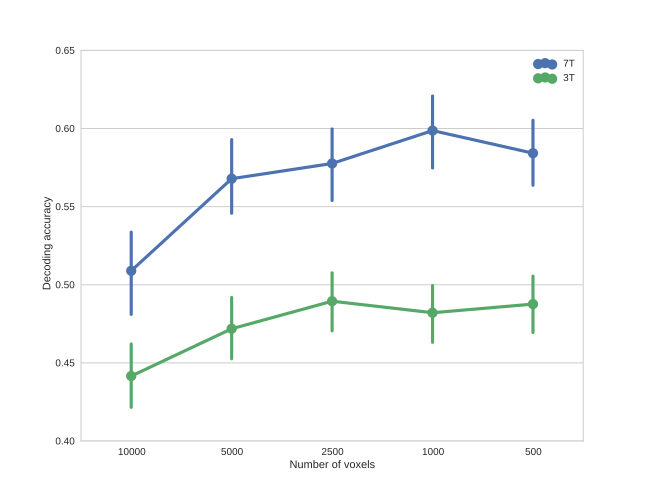
\includegraphics[width=\linewidth]{pics/nr_of_voxels_both}
	\caption{Mean decoding accuracy as a function of the included number of voxels for 3T and 7T. Error bars denote the bootstrapped 95\% confidence interval of the mean. The included voxels were the most stable ones i.e. their activity corresponding to each stimulus had the highest mean pairwise correlation across runs}
	\label{fig:voxelnr}
\end{figure}
 
 
 
%binary classification accuracy result, connect to casey/mitchel
\todo[inline]{potentially other nr of voxels, take avr across all runs for 3T and 7T}
\begin{figure}
	\centering
	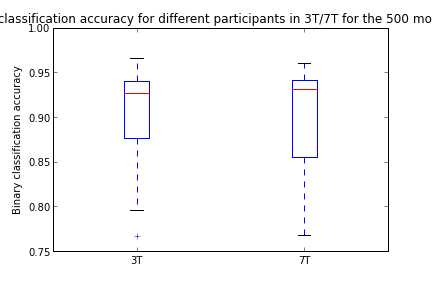
\includegraphics[width=\linewidth]{pics/binary_retrieval_accuracy}
	\caption{Binary retrieval classification accuracy for 3T and 7T}
	\label{fig:binretr}
\end{figure}
 
 
 
 
%correlation rankscore 3 and 7 incl. permutation analysis
\todo[inline]{potentially other nr of voxels, take avr across all runs for 3T and 7T,add permutation analysis}
\begin{figure}
	\centering
	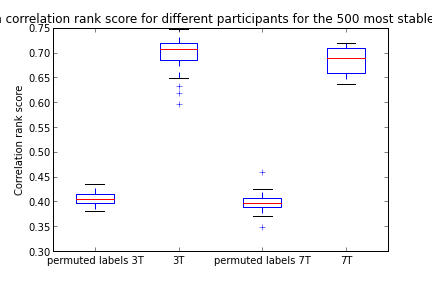
\includegraphics[width=\linewidth]{pics/correlation_rank_score}
	\caption{Correlation rank score for 3T and 7T}
	\label{fig:rankscore}
\end{figure}
 
 
 
 
 
%decoding(encoding) accuracy: 3 vs 7 (vs. plain decoding)
\todo[inline]{potentially other nr of voxels, take avr across all runs for 3T and 7T,add discriminative classifier baseline}
\begin{figure}
	\centering
	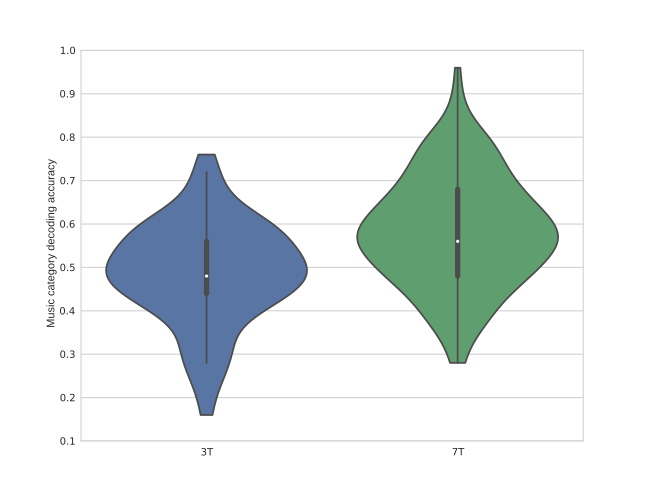
\includegraphics[width=\linewidth]{pics/decoding_accuracy}
	\caption{Decoding accuracy for 3T and 7T. A generative decoder was constructed by probabilistically inverting the encoding model.}
	\label{fig:decoder}
\end{figure}

\missingfigure{model validation on the movie}

\section*{Discussion}

\todo[inline]{7T doesnt matter -- stay cheap}

\todo[inline]{decode(encode(fmri)) vs. plain decoding}

\todo[inline]{naturalistic validation is now mandatory}


\section*{Author contributions}
%In order to give appropriate credit to each author of an article, the
%individual contributions of each author to the manuscript should be detailed
%in this section. We recommend using author initials and then stating briefly
%how they contributed.

MB performed the analysis and wrote the manuscript.
JSG contributed to the manuscript.
MH contributed to the manuscript.

\todo[inline]{describe author contributions}

\section*{Competing Interests}
No competing interests were disclosed.

\section*{Grant Information}

This research was, in part, supported by the German Federal Ministry of
Education and Research (BMBF) as part of a US-German collaboration in
computational neuroscience (CRCNS; awarded to James Haxby, Peter Ramadge, and
Michael Hanke), co-funded by the BMBF and the US National Science Foundation
(BMBF 01GQ1112; NSF 1129855).  Work on the data-sharing technology employed for
this research was supported by US-German CRCNS project awarded to
Yaroslav~O.~Halchenko and Michael~Hanke, co-funded by the BMBF and the US
National Science Foundation (BMBF 01GQ1411; NSF 1429999).  Michael Hanke was
supported by funds from the German federal state of Saxony-Anhalt, Project:
Center for Behavioral Brain Sciences.

\todo[inline]{add any financial support}

\section*{Acknowledgements}
%This section should acknowledge anyone who contributed to the research or the
%article but who does not qualify as an author based on the criteria provided
%earlier (e.g. someone or an organisation that provided writing assistance).
%Please state how they contributed; authors should obtain permission to
%acknowledge from all those mentioned in the Acknowledgements section.  Please
%do not list grant funding in this section (this should be included in the
%Grant information section - See above).

We are grateful to Michael Casey\ldots

\todo[inline]{express gratitude}

\bibliography{references}
\end{document}

% vim: textwidth=80 colorcolumn=81
